\documentclass[conference]{IEEEtran}
%\IEEEoverridecommandlockouts
% The preceding line is only needed to identify funding in the first footnote. If that is unneeded, please comment it out.
\usepackage[utf8]{inputenc}
\usepackage[T1]{fontenc}
\usepackage{hyperref}
\hypersetup{colorlinks=true,urlcolor=black,linkcolor=black,citecolor=black}
\usepackage{subfig}
\renewcommand{\sectionautorefname}{Section}
\usepackage{enumitem}
\usepackage{balance}
\usepackage{xcolor}
\usepackage{graphicx}
\usepackage{booktabs}
\usepackage{adjustbox}
\usepackage{multirow}
\usepackage{comment}
% \usepackage{subfigure}
% \usepackage{subfig}
\usepackage{threeparttable}
%\usepackage{siunitx}
\usepackage{microtype}
\usepackage{relsize,xspace}
\usepackage{cite}
\usepackage{textcomp}
\usepackage{mdframed}
\usepackage{framed}

%use the following command to DISABLE all to do notes and comments
%\usepackage[disable]{todonotes}
%use the following command to ENABLE all to do notes and comments
% \usepackage[]{todonotes}

% \newcommand{\tom}[1]{\todo[color=blue!40, inline]{\footnotesize{Tom: #1}}}
% \newcommand{\alex}[1]{\todo[color=orange!40, inline]{\footnotesize{Alex: #1}}}
% \newcommand{\john}[1]{\todo[color=green!40, inline]{\footnotesize{John: #1}}}
% \newcommand{\ahmed}[1]{\todo[color=purple!40, inline]{\footnotesize{Ahmed: #1}}}


\def\BibTeX{{\rm B\kern-.05em{\sc i\kern-.025em b}\kern-.08em
    T\kern-.1667em\lower.7ex\hbox{E}\kern-.125emX}}

\newcommand{\variants}{\textit{Variants}}
\newcommand{\pullrequestsmlvfv}{\ensuremath{\textit{PullRequest}_\textit{MLV-FV}}\xspace}
\newcommand{\pullrequestsfvmlv}{\ensuremath{\textit{PullRequest}_\textit{FV-MLV}}\xspace}
\newcommand{\pullrequestsfvfv}{\ensuremath{\textit{PullRequest}_\textit{FV-FV}}\xspace}
\newcommand{\StartingCommits}{\ensuremath{\textit{StartingCommits}}\xspace}
\newcommand{\StartingCommitsCdLOC}{\ensuremath{\textit{StartingCommits}_\textit{cdLOC}}\xspace}
\newcommand{\pullrequestscommlvfv}{\ensuremath{\textit{PullRequestsCom}_\textit{MLV-FV}}\xspace}
\newcommand{\pullrequestscomfvmlv}{\ensuremath{\textit{PullRequestsCom}_\textit{FV-MLV}}\xspace}
\newcommand{\DirectPullCom}{\ensuremath{\textit{DirectPullCom}_\textit{MLV-FV}}\xspace}
\newcommand{\VariabilityPercentage}{\ensuremath{\textit{VariabilityPercentage}}\xspace}
\newcommand{\VariabilityPercentageloc}{\ensuremath{\textit{VariabilityPercentage}_\textit{cdLOC}}\xspace}
\newcommand{\UniqueCom}{\ensuremath{\textit{UniqueCom}}\xspace}
\newcommand{\UniqueCdLOC}{\ensuremath{\textit{Unique}_\textit{cdLOC}}\xspace}
\newcommand{\MergedCom}{\ensuremath{\textit{MergedCom}}\xspace}
\newcommand{\MergedCdLOC}{\ensuremath{\textit{MergedCdLOC}}\xspace}

\newcommand{\TotalDevMLV}{\ensuremath{\textit{TotalDevMLV}}\xspace}
\newcommand{\TotalDevFV}{\ensuremath{\textit{TotalDevFV}}\xspace}
\newcommand{\CommonDevs}{\ensuremath{\textit{CommonDevs}}\xspace}
\newcommand{\TotalDevs}{\ensuremath{\textit{TotalDevs}}\xspace}
\newcommand{\Duration}{\ensuremath{\textit{Duration}}\xspace}
\newcommand{\ForkVariantBacklog}{\ensuremath{\textit{ForkVariantBacklog}}\xspace}
\newcommand{\Inactivity}{\ensuremath{\textit{Inactivity}}\xspace}
\newcommand{\Category}{\ensuremath{\textit{Category}}\xspace}
\newcommand{\Description}{\ensuremath{\textit{Description}}\xspace}

\definecolor{Mycolor2}{HTML}{00F9DE}

\newcommand{\secref}[1]{Section~\ref{#1}}
\newcommand{\figref}[1]{Fig.~\ref{#1}}
\newcommand{\Figref}[1]{Figure~\ref{#1}} %use if at beginning of sentence
\newcommand{\tabref}[1]{Table~\ref{#1}}
\newcommand{\lstref}[1]{Listing~\ref{#1}}

\newcommand{\compactlist}{\setlength{\itemsep}{0pt} \setlength{\parskip}{0pt}}
\newcommand\parhead[1]{\vspace{.26mm}\noindent\textbf{{#1}}.}

\newcommand{\jb}[1]{{\textsf{John}[\smaller\sffamily\color{blue} #1}]}
\newcommand{\tm}[1]{{\textsf{Tom}[\smaller\sffamily\color{red} #1}]}
\newcommand{\ad}[1]{{\textsf{Decan}[\smaller\sffamily\color{Mycolor2} #1}]}
\newcommand{\az}[1]{{\textsf{Ahmed}[\smaller\sffamily\color{orange} #1}]}
\newcommand{\sd}[1]{{\textsf{Serge}[\smaller\sffamily\color{pink} #1}]}

\newcommand{\gh}{\textsf{GitHub}\xspace}
\newcommand{\gl}{\textsf{GitLab}\xspace}
\newcommand{\bb}{\textsf{BitBucket}\xspace}
\newcommand{\np}{\textsf{npm}\xspace}
\newcommand{\scp}{\textit{SCP}\xspace}
\newcommand{\go}{\textsf{Go}\xspace}
\newcommand{\js}{\textsf{JavaScript}\xspace}

\newcommand{\npm}{{the \np package distribution platform}\xspace}
%\newcommand{\tb}[1]{}
%\newcommand{\sn}[1]{}
%\newcommand{\jb}[1]{}
\newcommand{\note}[1]{{\color{red}[NOTE: #1]}}

\begin{document}

\title{An Empirical Investigation of Forks as Variants in the npm Package Distribution}


\author{\IEEEauthorblockN{John Businge,\IEEEauthorrefmark{1}
		Alexandre Decan,\IEEEauthorrefmark{2}
	Ahmed Zerouali,\IEEEauthorrefmark{3} and
	Tom Mens\IEEEauthorrefmark{2}}
	\IEEEauthorblockA{\IEEEauthorrefmark{1}University of Antwerp, Antwerp, Belgium}
	\IEEEauthorblockA{\IEEEauthorrefmark{2}University of Mons, Mons, Belgium}
	\IEEEauthorblockA{\IEEEauthorrefmark{3} Vrije Universiteit Brussels, Brussels, Belgium}
	}



\maketitle

\begin{abstract}
Software developers often need to create variants to account for different customer segments. These variants have common code base but also comprise of variant specific code. A common strategy is to clone (or fork) an existing app and then adapt it to the new requirements. This form of reuse has been enhanced with the advent of social-coding platforms, such as \gh and package distribution platforms like \np: \gh offer facilities for forking, pull requests, and cross-project traceability. \np offers facilities of managing package release dependencies and dependents on the distribution platform. Little is known about the maintenance practices of the variants.
In this study we perform an exploratory investigation on the evolution variants focusing on their technical aspects. We collected variants from the \js ecosystem, whose sources are hosted on \gh, having their package releases on \npm. We have identified a significant number of variants from the \js ecosystem. We have also observed that, compared to their mainline counterparts, we find that variants do have a significant number of package releases, package dependencies, dependent packages and dependent projects.

%Social coding platforms like \gh and package distribution platforms like \np have substantially improved both code reuse and collaborative development. The two have provided a huge bazaar of software projects and components that can be reused through forking and package dependencies, respectively. \gh comprises a number of software ecosystems that form
\end{abstract}

\begin{IEEEkeywords}
software variants, npm, depandencies, software ecosystems
\end{IEEEkeywords}

\section{Introduction}
Today, developing quality software faster developers rely on code reuse and distributed collaborative development tools. Social coding platforms like \gh have substantially improved  both code reuse and collaborative development, providing a huge bazaar of software projects and components that can be reused through explicit project dependencies or forking of software repositories. This is supported by various automated facilities such as pull requests, dependency management tools, issue tracking systems (e.g. \textsf{JIRA}), source code review tools (e.g., \textsf{Gerrit}), Q\&A services (e.g. \textsf{StackOverflow}), continuous integration tools (e.g., \textsf{Travis CI}), and package distribution managers (e.g., \np). Social coding platforms comprise a number of social software ecosystems i.e., large collections of interdependent software components that are maintained by large and geographically distributed communities of collaborating contributors~\cite{lungu:2008,decan:2017}.
The ecosystems form large socio-technical networks of technical and social components that interact with each other on top of common software and hardware platforms.
The unprecedented growth of these ecosystems relies on substantial software reuse using different methods and tools \cite{mojica2014large}.

Our research focuses on the phenomenon of forking in particular in the software ecosystems.
Forking a software repository (referred to as the \textit{mainline}, i.e., the original repository) produces several \textit{forked} repositories.
Two types of forks exist~\cite{Zhou:2020}. \textit{Social forks} are created for isolated development, but with the goal of contributing back to the mainline.
\textit{Variant forks} are created for splitting off a new development branch, often to steer the development into another direction than the mainline, without the intention to contribute back.
Variant forking may split the core development team and always splits the contributing community.
Variant forking creates variants of the mainline repository, which share common code, but also contain variant-specific code that needs to be maintained.
A mainline repository together with all its variant repositories can be seen as a software product family, inspired by the notion of \textit{software product lines}~\cite{berger.ea:2020:emse}.
The  family members have software artefacts in common, but also contain artefacts that are specific to one or multiple variants.

\begin{figure}[ht]
  \begin{center}
  \small
  %\vspace{-10pt}
    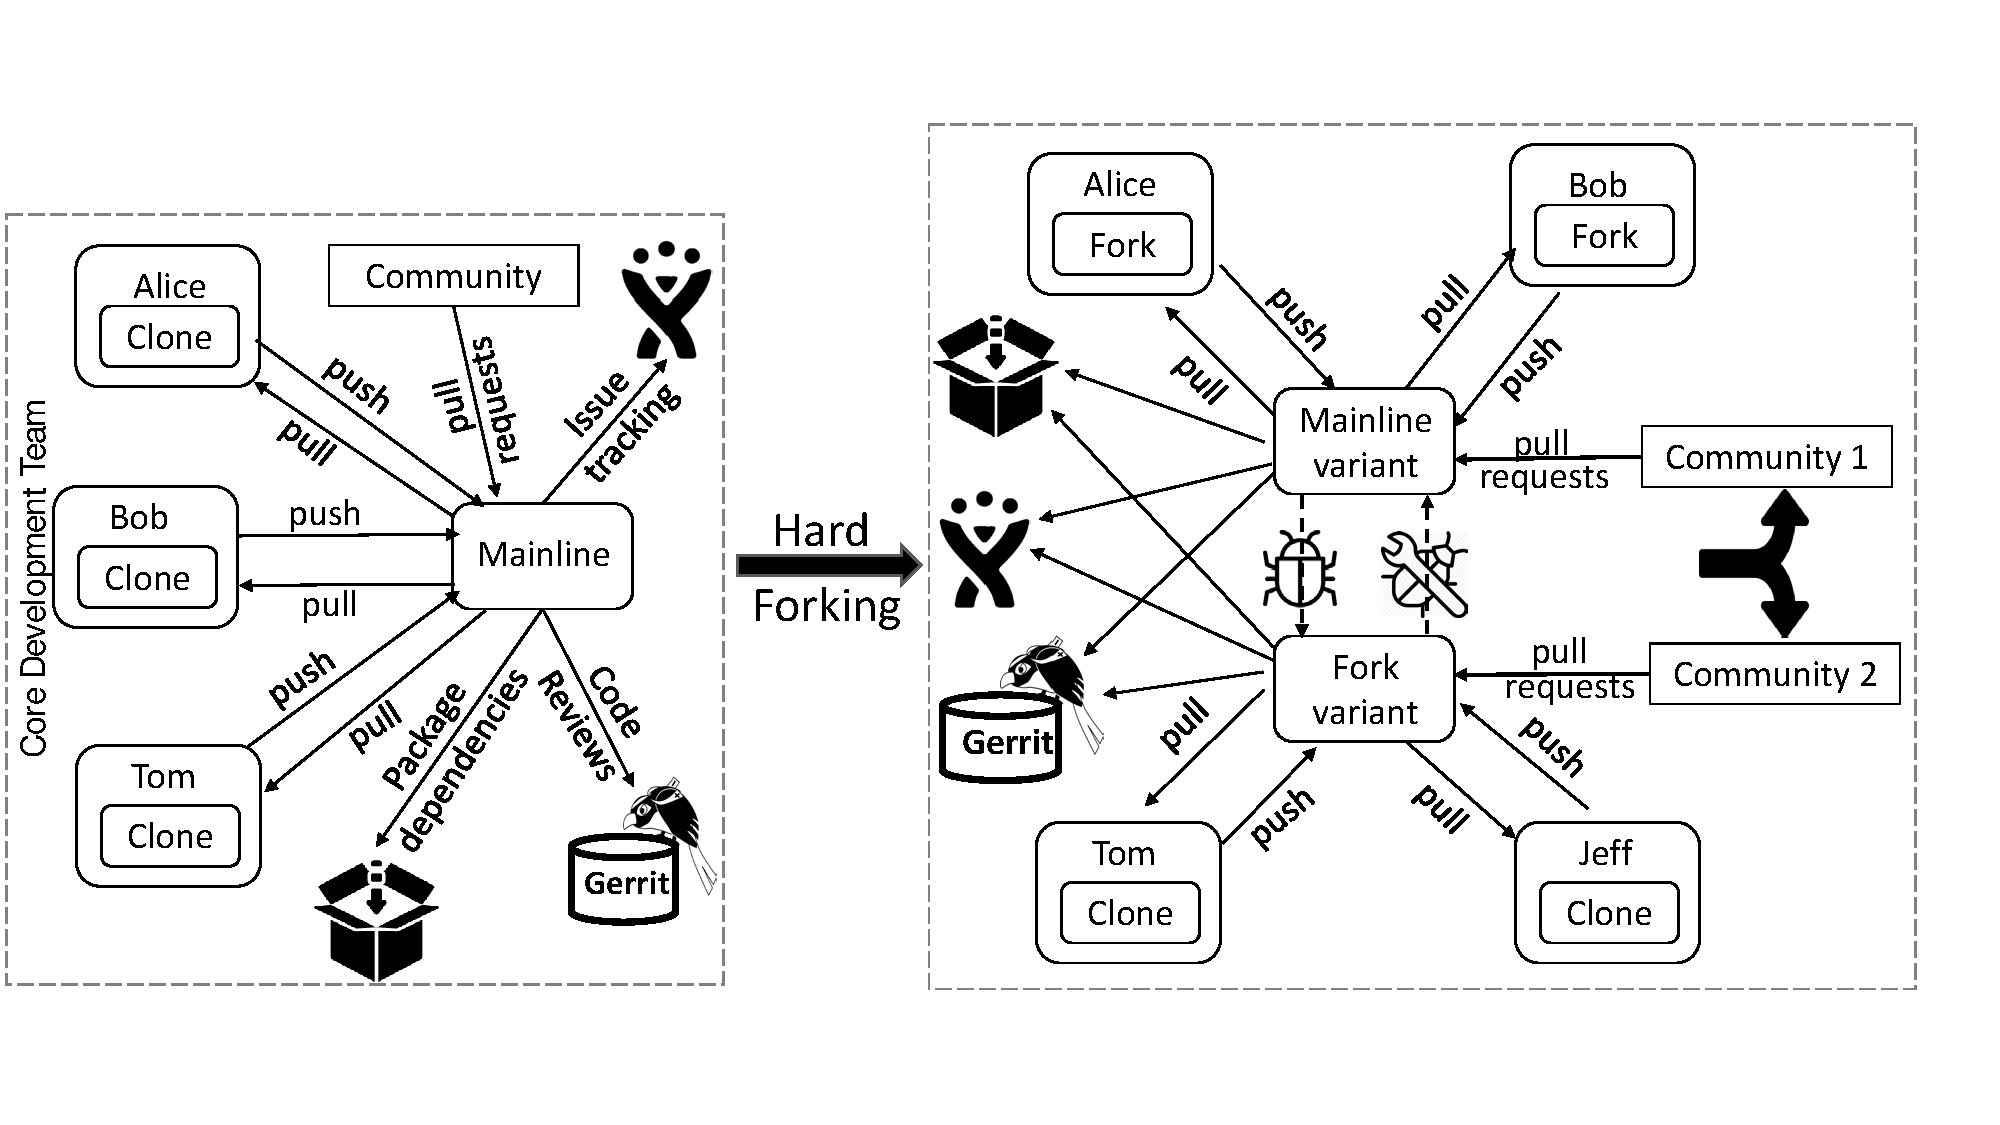
\includegraphics[width=0.5\textwidth]{figures/Collaboration.pdf}
  \end{center}
  \caption{Maintenance of a software repository before (left) and after (right) variant forking.}
  %\vspace{-10pt}
  \label{fig:forking}
\end{figure}

Figure~\ref{fig:forking} illustrates the development activities on a repository before and after variant forking.
On the left, we can see three core developers (Alice, Bob and Tom) that have write access to the mainline repository.%\tom{If Alex, Bob and Tom have write access, then why do they have to go through the pull/push mechanism? Isn't it also possible or them to do direct commits?} 
  \jb{push and pull is actually performing the direct commits in a shared repository}
The community interacts with the mainline by sending pull requests, submitting issues and conducting change reviews.
After variant forking, shown on the right, the core developers are split into two.
Alice and Bob remain with the original mainline, while Tom is joined by a new developer Jeff to maintain a new fork variant in parallel to the mainline project.
This parallel development between mainline and variant has split the contributing community. New contributors could decide to contribute to the mainline or the variant, for instance depending on which one is more open to accommodate newcomers.
Furthermore, as a result of parallel maintenance, developers in one of the projects may identify and fix bugs in shared artefacts.
%\tom{Why would there be any shared artefacts if the split/fork is not a social fork?} 
\jb{they have shared artefacts since they share a common code base and they are still interconnected through traceability links}
Developers in each variant of the family are not obligated to contribute back but if they wish, the fixes could be propagated to other members of the family to avoid effort duplication.
%\tom{Why would there be any incentive to propagate fixes if the variant forks are not social forks?} \jb{bug fixed appearing in shared artefacts could be shared among the families although the developers are not obligated propagate back. For example is the family is owned by the same company. If the developers were notified of the interesting changes that have taken place in the other variants, they would integrate them into their own variants. This helps avoid duplication of efforts.}

There have been many studies on variant forks. However, most of these studies were carried out on \texttt{SourceForge}~\cite{Linus:2012Perspectives,Gregorio:2012,Viseur:2012Forks,Linus:2013CodeForking,Laurent:2008,Linus:2011ToFork}, before the advent of social coding platforms such as \gh.
We have found only two studies that investigated variant forks on \gh~\cite{businge2018appfamilies,Zhou:2020}.
While the pre-\gh studies report controversial perceptions around variant forks~\cite{Chua:Forking:2017,Dixion:2009Forks,Ernst:2010,Linus:2011ToFork,Linus:2014Hackers,Raymond:Cathedral:2001}, Zhou et al.~\cite{Zhou:2020} reports that these perceptions have changed with the advent of \gh. Jiang et al.~\cite{Lo:2017} state that, although forking is controversial in traditional open source software (OSS) communities, it is actually encouraged as a built-in feature in \gh. Jiang et al. ~\cite{Lo:2017} further reports that developers fork repositories to submit pull requests, fix bugs, add new features and keep copies (social forks).
Zhou et al.~\cite{Zhou:2020} also report that many variant forks actually start as social forks.

While numerous studies have investigated variant forking, we are not aware of any study that has investigated the socio-technical specificities of these variant forks that are part of \textbf{software ecosystems}.
Our research therefore aims at empirically studying the evolution of \textbf{software families} (a subset of software ecosystems), that are composed of variant project repositories by investigating their socio-technical aspects. Specifically, we would like to investigate evolution socio-technical specificities of the software families in the \js ecosystem whose repositories are hosted on \gh.
For the social aspects, it would be interesting to look at the interaction and collaboration between communities involved in the mainline and variants.
For example, finding out how different are collaborations with respect to who forked and how the fork has been created?
For the technical aspects, ecosystems are often characterised by numerous dependency relationships between the packages on software package distribution platforms~\cite{decan:2016:ECSAW}. 
As a result of parallel development of the mainline and its variants, while offering similar functionality, it would be interesting to investigate if their dependent projects migrate from one variant of the required package to another in a family.
%As a preliminary step, this paper investigates the socio-technical aspects of forking in the \npm, the largest collection of \js packages. 

Before we can proceed to state our goal and research questions of this study let us first discuss the terminologies we will use in our analysis and also give a concrete example: 

\begin{itemize}
    \item \textbf{Package.} One that is distributed in a package manager (e.g., \np).
    
    \item \textbf{Mainline.} A repository that is hosted on \gh 
    whose package releases are distributed on \npm.

    \item \textbf{Variant.} A fork repository of the \textbf{mainline} that is hosted on \gh whose package is distributed on \npm.

    \item \textbf{Software family.} As set of two or more repositories (the mainline and its variants) that are hosted on \gh with the package releases of both mainline and its variants distributed on \npm.

    %\ad{(for what follows) do we really need mathematical notations, and a true formalisation of these concepts? It seems we are not even using the notations in the RQs. }
    %\tm{I agree that for a short 4-page paper it is not necessary to have formal definitions. Especially if we do not use them later on.}
    
    \item \textbf{Release.} These are one or more releases of a package distributed on \npm.
    %Let $E$ be a package distribution, i.e., a set of packages. Given a package $p\in E$, releases($p$) denotes the set of releases of $p$. Every release $r\in$ releases ($p$) has a release date $r_{date}$ and a version $r_{version}$.

     \item \textbf{Dependency.} These are the packages that a given release of a package depends on.
     %A release $r$ has a (potentially empty) set $r_{deps}$ of dependencies. A dependency $d \in r_{deps}$ is defined as a pair($d_{target}$, $d_{constraint}$) composed of a target package $d_{target} \in E$ and a dependency constraint $d_{constraint}$ over the releases in releases ($d_{target}$).

    \item \textbf{Dependent.}  A package $A$ depending on a package $B$ is a ``dependent package of $B$''. By definition, both $A$ and $B$ are distributed in a package distribution platform. A project is a repository in which a package is developed, but not necessarily distributed in a package distribution platform. By extension, a project $A$ depending on a package $B$ is a ``dependent project''. In this case, $B$ is distributed in a package distribution platform, but not necessarily $A$.

\end{itemize}

To put the the presented terminologies in perspective, let us present a concrete example of a software family. 
The mainline repository \texttt{creationix/wheat} is hosted on \gh (with a total of 136 forks and six contributors), is a blog engine for coders written in \texttt{node.JS}. 
The mainline and 2 of 136 forks (\texttt{sun11/wheat} and \texttt{frodare/barley}) have their package releases on \npm. 
In Table~\ref{tab:example} we present statistics corresponding to the package releases, package dependencies, dependent packages and dependent projects for three repositories in the software family.
For example, the mainline repository has 13 package releases, 77 package dependencies, 2 dependent packages and 23 dependent projects.

\begin{table}[ht]
\begin{center}
% \small
\caption{Count of the mainline and variants releases, dependencies, dependent packages and dependent projects. M = mainline and F = fork.}
\label{tab:example}
\begin{tabular}{l r r r r } 
 \hline
 &releases & dependencies & \shortstack{dependent \\ packages} & \shortstack{dependent \\ projects} \\ \hline
 creationix/wheat (M)  &13 & 77 & 2&23 \\ 
 frodare/barley (F)    &1 & 8 & 0 & 0 \\ 
 sun11/wheat (F)       &1 & 6 & 1 & 1 \\ 
 \hline
\end{tabular}
\end{center}
\end{table}
%\tm{A concrete example is at its place here.}

\section{Goal and Research Questions}
As stated earlier, since this research is the first of its kind in studying socio-technical specificities of the variant forks that are part of \textbf{software ecosystems}. In this study, our goal is to perform an exploratory investigation on the evolution of variants focusing on their technical aspects. We mined repositories from the \js ecosystem, whose sources are hosted on \gh, having their package releases on \npm. This allows us identify the software families as well as studying the technical aspects of those families.
Below we state the four research questions for our study.
\begin{itemize}
\item[\textbf{$RQ_0$}] \textit{How prevalent are software families in \js ecosystem on \gh?}
%\tom{It needs to be made clear what is meant by "software families in \np", since before you only talked about software families in social coding platforms, and more specifically in \gh. This link needs to be made really clear.}
We would like to determine whether software families exist in software ecosystems. If software families rarely exist, results about their social-technical evolution may not be statistically significant.
%\tm{You should not confuse a research GOAL with a research QUESTION. Typically a research goal is much higher level. According to the goal-question metric (GQM) paradigm, you can derive questions from goals, and then answer these questions by means of metrics.}
%\ad{I'm missing the motivation for the three following RQs. If it's mainly exploratory, then we should state it, and explain why these questions are worth to consider (i.e., how the answer helps).}
\item[\textbf{$RQ_1$}] \textit{How do the distributions of package releases in mainlines and their variants compare to each other?}
This RQ will help us determine if mainlines and variants are continuously maintained. A package that is continuously distributing new releases means that it introducing new features and address issues raised by its users.

%\tm{Why is it important or relevant to know if they are continuously maintained?}
%Do most variants have one-off releases?\tm{What do you mean by one-off releases? This term is not explained neither introduced anywhere...}

\item[\textbf{$RQ_2$}] \textit{How do the distributions of package dependencies in mainlines and their variants compare to each other?}
This RQ will help us determine if the mainlines and their variants in depend on other packages in the \np ecosystem. If they have dependencies on other packages, then studying the dependency relationships between the packages in the software families and other packages would be interesting.
%\tm{Unclear what is meant by "members in the software families depend on other packages}

\item[\textbf{$RQ_3$}] \textit{Do the variant packages have dependent packages\,/\,projects?}
This RQ will help us determine other packages\,/\,projects in the ecosystem that depend on the variant projects.
Since they are forks of the mainline, it would be interesting to find other packages are interested depending on variants as opposed to their mainline counterparts offering similar functionality.

%variants that have more dependent packages\,/\,projects. Having dependent packages\,/\,projects means that other users are interested in them.
\end{itemize}
%\tm{The RQs, their motivation, and the overall research goal in which these questions fit need to be explained much better...}


\section{Methods and Dataset}
\label{sec:method}
According to the 2020 Stack Overflow Developer Survey\footnote{https://insights.stackoverflow.com/survey/2020} to which over 65,000 developers participated, \js is one the most commonly used programming language (67.7\% of all respondents make use of \js).




%\textbf{Dataset}.
 Our dataset of \gh repositories from the \js ecosystem and their corresponding \np packages, dependents and dependencies were extracted from the \texttt{libraries.io} release 1.6.0 of January 12, 2020. We use the following heuristics to extract the mainline--variant pairs of the software families in the \js ecosystem on \gh: the repository $A$ is a variant of the repository $B$ if (1) the package releases of $A$ and $B$ are distributed on \np and (2) $A$ is a fork of $B$ on \gh.
%\tom{On \gh?} 
Since we focus on the \js ecosystem on \gh, we extracted software families whose repositories are hosted on \gh and their packages distributed on \np.
%\tm{This sentence comes much too late and is not sufficiently detailed.} 
For each mainline and its corresponding variants we collected their releases, dependencies and dependents (projects and packages).








\section{Results}
\label{sec:results}
\begin{figure}[htbp]
\vspace{-.3cm}
   \centering
    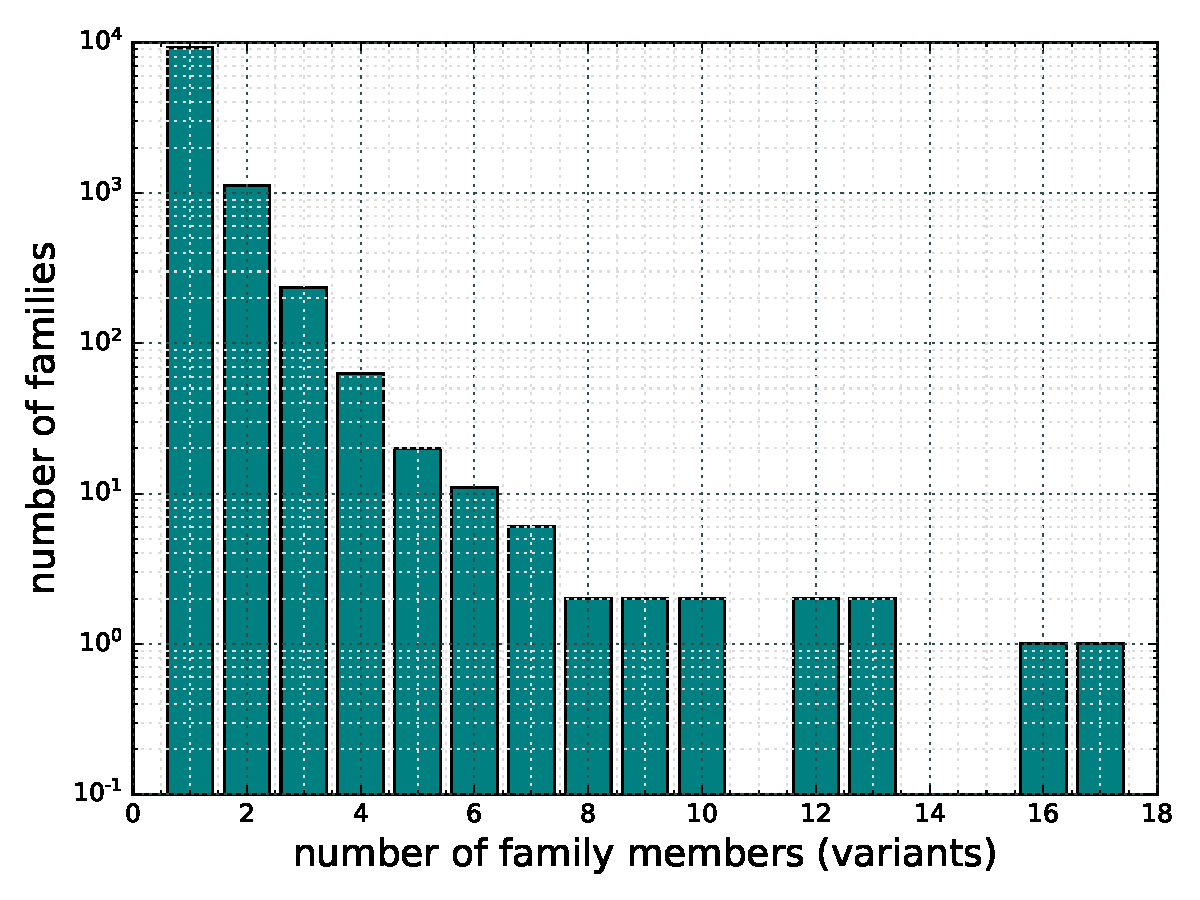
\includegraphics[scale=0.4]{figures/variants.pdf}
    \caption{Family size (number of variants in a family).}
    \label{fig:variants}
\end{figure}

\noindent
\textit{RQ0}: \textbf{How prevalent are software families?}

With this first RQ, we aim to determine if software families exist in software ecosystems. In the \js ecosystem we discovered 12,813 variants of the mainline and a total of 10,743 software families. In Figure~\ref{fig:variants} we present the distribution of the software families. On the y-axis we have the number of families and on the x-axis we have the number of variants in the families. For example, the first bar tells us that there are 9,280 families that contain only one variant. We also observe one family each containing as many as 16 and 17 variants, respectively. The results of RQ0 give us confidence that indeed software families exist in software ecosystems.

\begin{figure}[htbp]
\vspace{-.3cm}
   \centering
    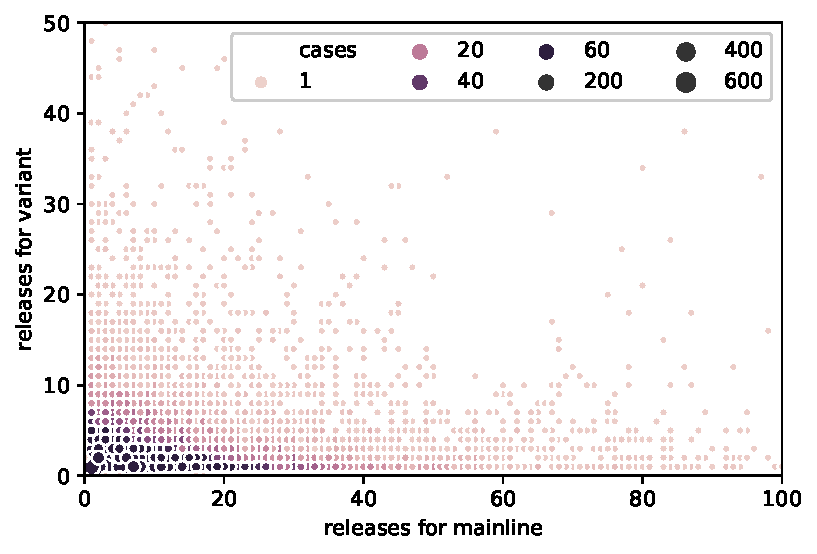
\includegraphics[scale=0.6]{figures/benevolj_releases.pdf}
    \caption{The distribution of the mainline versus variant package releases.}
    \label{fig:releases}
\end{figure}

\textit{RQ1}: \textbf{The distribution of package releases for mainlines versus variants.}

With this second RQ, we aim to ascertain if the mainlines and the variants are continuously maintained. 
In Figure~\ref{fig:releases} we present a scatter plot showing the distribution of releases for the variants versus the releases for the mainlines. 
On the x-axis we have the number of releases for the mainlines and on the y-axis we have the number of releases for the variants. 
The color of the data points in the graph represent the number cases for the mainlines\,/\,variants. 
For example, the data points on the top left of the graph tell us that there are some variants that have more releases compared to their mainline counterparts. 
This implies the variants are being maintained more than their mainline counterparts.
The data points on the bottom right tell us that there are a number of mainlines having many releases compared to their variant counterparts. 
Overall, we observe more mainlines being maintained compared to their variant counterparts.
However, we also observe a significant amount of variants being maintained. 
This is interesting since developers variants did not make a one off package distribution; they are continuously distributing new releases of their package. 

\begin{figure}[htbp]
\vspace{-.3cm}
   \centering
    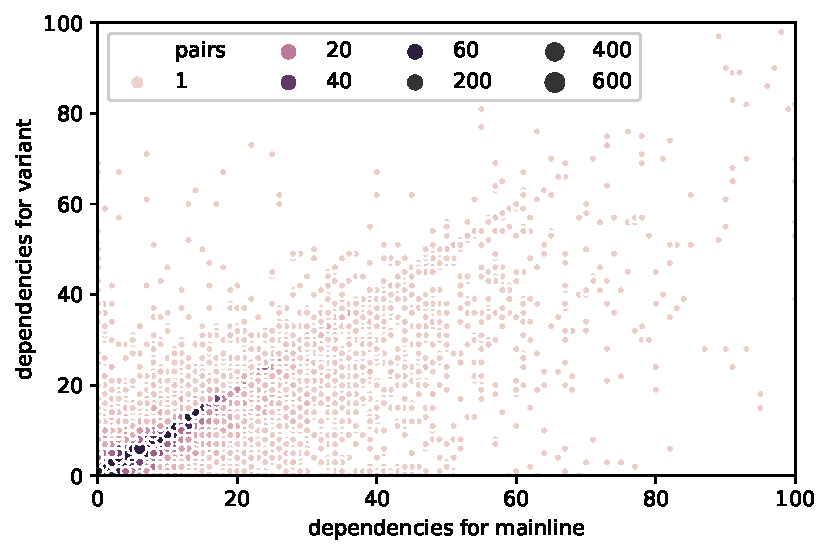
\includegraphics[scale=0.6]{figures/benevolj_dependencies.pdf}
    \caption{The distribution of the mainline versus variant package dependencies.}
    \label{fig:dependencies}
\end{figure}


\textit{RQ2}: \textbf{The distribution of package dependencies for the mainlines versus variants.}

With this RQ, we want to ascertain the frequency of package dependencies on other packages for the mainlines and the variants in the software families. 
In Figure~\ref{fig:dependencies} we present a scatter plot showing the distribution of the package dependencies of the variants versus the dependencies of the mainline.
On the x-axis we have the number of dependencies of the mainline. 
On the y-axis we have the number of dependencies of the variant.
The color of the data points in the graph represent the number cases for the mainlines\,/\,variants.
For example, on the top right of the graph we see a few scattered points single case variants telling us that there are a few variants that have many dependencies compared to the variant counterparts.
We also see many scattered single case mainlines having many dependencies compared to their variant counterparts. 
overall, we observe the mainlines having more dependencies compared to their variant counterparts.

\begin{figure*}%
    \centering
    \subfloat[Packages]{{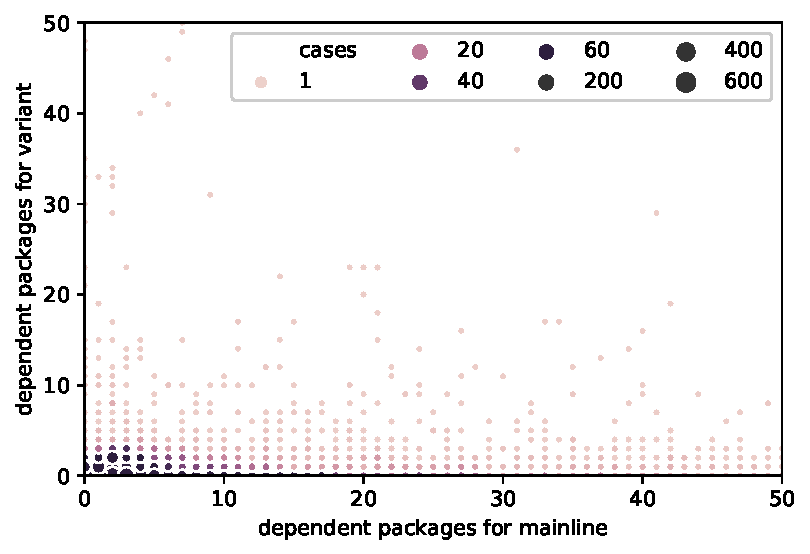
\includegraphics[width=8cm]{figures/dependents} }}%
    \qquad
    \subfloat[Projects]{{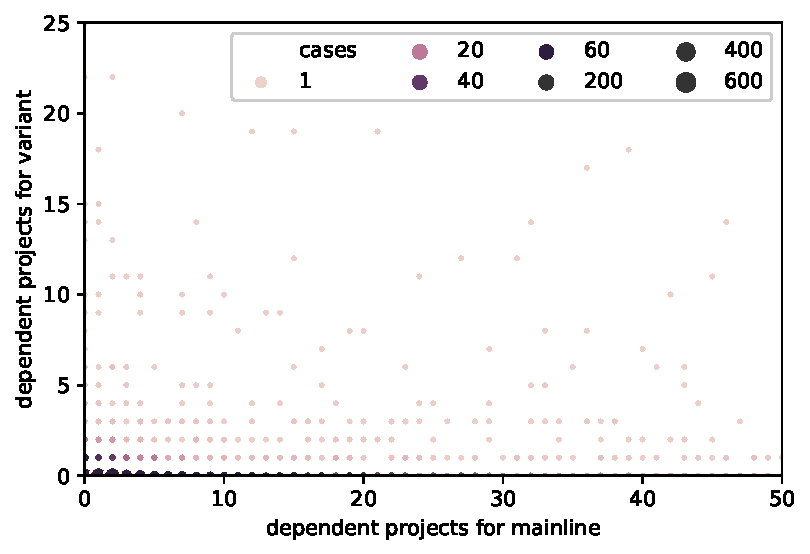
\includegraphics[width=8cm]{figures/benevolj_projects} }}%
    \caption{Distribution of dependent packages and dependent projects for the mainline versus variants.}%
    \label{fig:packages_and_projects}%
\end{figure*}


\begin{figure*}%
    \centering
    \subfloat[ Mainlines]{{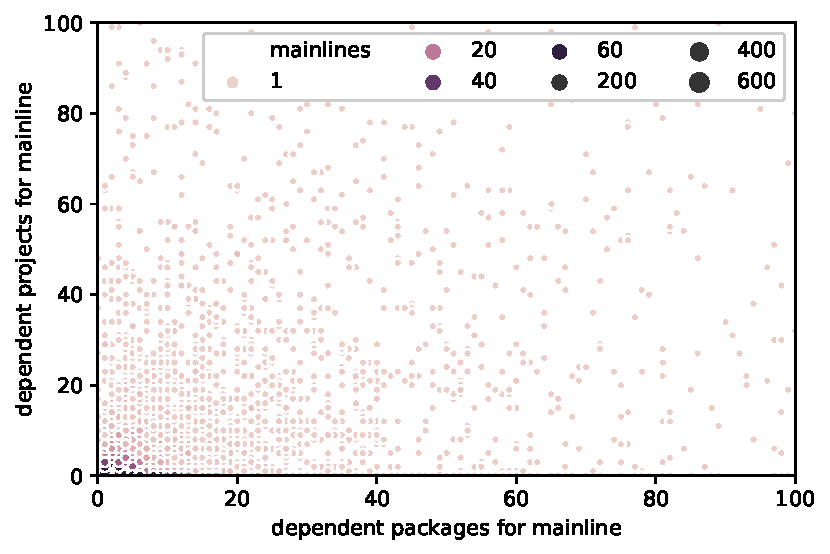
\includegraphics[width=8cm]{figures/benevolj_dependents_mainline.pdf} }}%
    \qquad
    \subfloat[ Variants]{{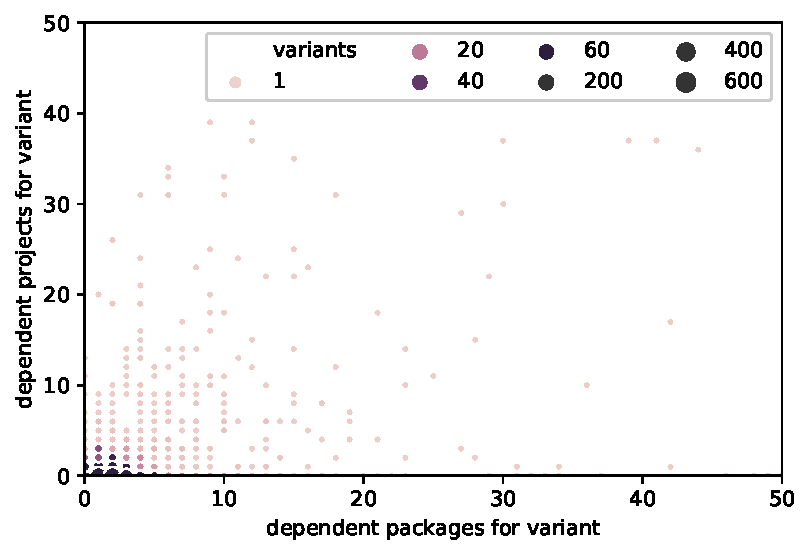
\includegraphics[width=8cm]{figures/benevolj_dependents_variant.pdf} }}%
    \caption{Distribution of dependent packages versus dependent projects for mainlines and variants.}%
    \label{fig:mainline_variants_packages}%
\end{figure*}

\textit{RQ3}: \textbf{The distribution of dependent packages and projects of the mainlines and variants.}

In this RQ we are interesting in observing if other packages\,/\,projects in the ecosystem depend on the variants.
In Figure~\ref{fig:packages_and_projects} we present the scatter plots showing the distribution of the dependent packages (Figure~\ref{fig:packages_and_projects}-(a)) and dependent projects (Figure~\ref{fig:packages_and_projects}-(b)) for the variants versus mainlines.
The x-axes represent the number of dependent packages for the mainline and number of dependent projects for the variants, respectively.
The y-axes represent the number of dependent packages for the variants and number of dependent projects for the variants, respectively.
The color of the data points in the graph represent the number cases for the mainlines\,/\,variants.
Looking at Figure~\ref{fig:packages_and_projects}-(a), we observe that most of the data points are concentrated on the x-axis. 
This implies that there are very many mainline variants having many dependent packages compared to their variant counterparts.
We observe the same trend for the dependent projects in Figure~\ref{fig:packages_and_projects}-(b).
In both Figure~\ref{fig:packages_and_projects}-(a) and Figure~\ref{fig:packages_and_projects}-(b), we observe that most variants have $<10$ dependent packages\,/\,projects. 
This is still interesting since it implies that some developers do depend on the variants as opposed to their mainlines counterparts offering similar functionality.


\section{Conclusion}
\label{sec:conclusion}
%We carried out an empirical analysis of forks variants, with the ultimate goal of investigating the social-technical specificities of the software families in the \js ecosystem whose repositories are hosted on \gh. 
As a preliminary step, we performed an exploratory investigation on the evolution variants focusing on their technical aspects. We mined repositories from the \js ecosystem, whose sources are hosted on \gh, having their package releases on \npm.
We identified a significant number of variants from the \js ecosystem. We have also observed that, compared to their mainline counterparts, we find that variants do have a significant number of package releases, package dependencies, dependent packages and dependent projects.

As future work, we plan to use the current results to carry out an extensive investigation on the social-technical specificities of the software families in the \js ecosystem whose repositories are hosted on \gh. 




%\balance
% references section

\bibliographystyle{IEEEtran}
\bibliography{biblio}


\end{document}
